\documentclass[11pt]{article}
\usepackage[a4paper,margin=19mm]{geometry}
\usepackage[no-math]{fontspec}
\setmainfont{Latin Modern Roman}[SmallCapsFont=Latin Modern Roman Caps]
\usepackage{amsmath,amssymb,amsthm,mathtools,amscd,verbatim,xcolor,graphicx,hyperref}
\hypersetup{hidelinks}
\numberwithin{equation}{section}
\newtheorem{theorem}{Theorem}[section]
\newtheorem{lemma}[theorem]{Lemma}
\newtheorem{proposition}[theorem]{Proposition}
\newtheorem{corollary}[theorem]{Corollary}
\newtheorem{claim}[theorem]{Claim}
\newtheorem{fact}[theorem]{Fact}
\newtheorem{conjecture}[theorem]{Conjecture}
\theoremstyle{definition}
\newtheorem{definition}[theorem]{Definition}
\newtheorem{example}[theorem]{Example}
\newtheorem{remark}[theorem]{Remark}
\newtheorem{question}[theorem]{Question}
\theoremstyle{plain}
\newcommand{\C}{\mathbb C}
\newcommand{\R}{\mathbb R}
\newcommand{\Q}{\mathbb Q}
\newcommand{\Z}{\mathbb Z}
\newcommand{\N}{\mathbb N}
\newcommand{\eee}{\mathrm e}
\newcommand{\cclass}[1]{\textsf{#1}}
\newcommand{\cproblem}[1]{\textsc{#1}}
\newcommand{\ie}{i.\,e.}
\newcommand{\Ie}{I.\,e.}
\newcommand{\eg}{e.\,g.}
\newcommand{\Eg}{E.\,g.}
\newcommand{\phd}{Ph.\,D.}
\newcommand{\msc}{M.\,S.}
\newcommand{\bsc}{B.\,S.}
\newcommand{\expref}[2]{\hyperref[#2]{#1~\ref{#2}}}
\newcommand{\expeqref}[2]{\hyperref[#2]{#1~\eqref{#2}}}
\newcommand{\exprefsilent}[2]{\hyperref[#2]{#1}}
\newcommand{\epfmtdoi}[1]{\href{https://doi.org/#1}{doi:#1}}
\emergencystretch=3em
\usepackage{etoolbox,bm}
\newcommand{\epfmt}[2]{\begingroup\def\TocNativeBibResult{\PackageError{toc-native-compat}{Unsupported bibliography type/record #1/#2}{Only exact source-observed finite records are allowed.}}\ifstrequal{#1}{arxiv}{\ifstrequal{#2}{1412.7392}{\def\TocNativeBibResult{\href{http://arxiv.org/abs/1412.7392}{arXiv:#2}}}{}}{}\ifstrequal{#1}{arxiv}{\ifstrequal{#2}{1702.03849}{\def\TocNativeBibResult{\href{http://arxiv.org/abs/1702.03849}{arXiv:#2}}}{}}{}\ifstrequal{#1}{arxiv}{\ifstrequal{#2}{1702.05575}{\def\TocNativeBibResult{\href{http://arxiv.org/abs/1702.05575}{arXiv:#2}}}{}}{}\ifstrequal{#1}{arxiv}{\ifstrequal{#2}{1707.03663}{\def\TocNativeBibResult{\href{http://arxiv.org/abs/1707.03663}{arXiv:#2}}}{}}{}\ifstrequal{#1}{arxiv}{\ifstrequal{#2}{1708.07114}{\def\TocNativeBibResult{\href{http://arxiv.org/abs/1708.07114}{arXiv:#2}}}{}}{}\ifstrequal{#1}{arxiv}{\ifstrequal{#2}{1710.00095}{\def\TocNativeBibResult{\href{http://arxiv.org/abs/1710.00095}{arXiv:#2}}}{}}{}\ifstrequal{#1}{arxiv}{\ifstrequal{#2}{1710.06261}{\def\TocNativeBibResult{\href{http://arxiv.org/abs/1710.06261}{arXiv:#2}}}{}}{}\ifstrequal{#1}{arxiv}{\ifstrequal{#2}{1801.02309}{\def\TocNativeBibResult{\href{http://arxiv.org/abs/1801.02309}{arXiv:#2}}}{}}{}\ifstrequal{#1}{arxiv}{\ifstrequal{#2}{1802.05431}{\def\TocNativeBibResult{\href{http://arxiv.org/abs/1802.05431}{arXiv:#2}}}{}}{}\ifstrequal{#1}{arxiv}{\ifstrequal{#2}{1802.08089}{\def\TocNativeBibResult{\href{http://arxiv.org/abs/1802.08089}{arXiv:#2}}}{}}{}\ifstrequal{#1}{arxiv}{\ifstrequal{#2}{1803.06573}{\def\TocNativeBibResult{\href{http://arxiv.org/abs/1803.06573}{arXiv:#2}}}{}}{}\ifstrequal{#1}{arxiv}{\ifstrequal{#2}{1805.01648}{\def\TocNativeBibResult{\href{http://arxiv.org/abs/1805.01648}{arXiv:#2}}}{}}{}\ifstrequal{#1}{arxiv}{\ifstrequal{#2}{1807.09382}{\def\TocNativeBibResult{\href{http://arxiv.org/abs/1807.09382}{arXiv:#2}}}{}}{}\ifstrequal{#1}{arxiv}{\ifstrequal{#2}{1812.06243}{\def\TocNativeBibResult{\href{http://arxiv.org/abs/1812.06243}{arXiv:#2}}}{}}{}\ifstrequal{#1}{arxiv}{\ifstrequal{#2}{1902.00996}{\def\TocNativeBibResult{\href{http://arxiv.org/abs/1902.00996}{arXiv:#2}}}{}}{}\ifstrequal{#1}{arxiv}{\ifstrequal{#2}{1903.08568}{\def\TocNativeBibResult{\href{http://arxiv.org/abs/1903.08568}{arXiv:#2}}}{}}{}\ifstrequal{#1}{arxiv}{\ifstrequal{#2}{1905.02313}{\def\TocNativeBibResult{\href{http://arxiv.org/abs/1905.02313}{arXiv:#2}}}{}}{}\ifstrequal{#1}{arxiv}{\ifstrequal{#2}{1905.12247}{\def\TocNativeBibResult{\href{http://arxiv.org/abs/1905.12247}{arXiv:#2}}}{}}{}\ifstrequal{#1}{arxiv}{\ifstrequal{#2}{1906.08530}{\def\TocNativeBibResult{\href{http://arxiv.org/abs/1906.08530}{arXiv:#2}}}{}}{}\ifstrequal{#1}{arxiv}{\ifstrequal{#2}{1908.04746}{\def\TocNativeBibResult{\href{http://arxiv.org/abs/1908.04746}{arXiv:#2}}}{}}{}\ifstrequal{#1}{arxiv}{\ifstrequal{#2}{1908.10859}{\def\TocNativeBibResult{\href{http://arxiv.org/abs/1908.10859}{arXiv:#2}}}{}}{}\ifstrequal{#1}{arxiv}{\ifstrequal{#2}{1909.05503}{\def\TocNativeBibResult{\href{http://arxiv.org/abs/1909.05503}{arXiv:#2}}}{}}{}\ifstrequal{#1}{arxiv}{\ifstrequal{#2}{1911.01469}{\def\TocNativeBibResult{\href{http://arxiv.org/abs/1911.01469}{arXiv:#2}}}{}}{}\ifstrequal{#1}{arxiv}{\ifstrequal{#2}{2002.04121}{\def\TocNativeBibResult{\href{http://arxiv.org/abs/2002.04121}{arXiv:#2}}}{}}{}\ifstrequal{#1}{arxiv}{\ifstrequal{#2}{math/0701886}{\def\TocNativeBibResult{\href{http://arxiv.org/abs/math/0701886}{arXiv:#2}}}{}}{}\TocNativeBibResult\endgroup}

%% Theory of Computing
%% File: v018a009.tex
%% Publication date: April 30, 2022
%% Authors: Zongchen Chen and Santosh S. Vempala
%
%
%
%

%

%
%

%
%
%
%
%
%
%
%
%
%
%
%
%
%
%
%
%
%
%
%
%
%
%
%

%



\usepackage{graphicx}

%
%
%
   %

    %
    %
    %
    %
    %
    %
    %
    %
    %
    %
    %
    %
    %
    %
    %
    %
    %
    %
    %
    %
    %
    %
    %
    %
    %
    %
    %
    %
    %

%
%
   %




\newcommand{\poly}{\mathrm{poly}}
\newcommand{\e}{\mathrm{e}}
\newcommand{\dif}{\mathrm{d}}
\newcommand{\pr}{\mathbb{P}}
\newcommand{\Exp}{\mathbb{E}}
\newcommand{\Var}{\mathrm{Var}}
\newcommand{\Cov}{\mathrm{Cov}}
\newcommand{\MI}{\mathrm{I}}
\newcommand{\Ind}{\mathbbm{1}}
\newcommand{\tr}{\mathrm{tr}}
\newcommand{\wt}{\mathrm{weight}}
\DeclareMathOperator*{\argmax}{arg\,max}
\newcommand{\norm}[1]{\left\lVert #1 \right\rVert}
\newcommand{\Po}{\mathrm{Poi}}
\newcommand{\wei}{W}
\newcommand{\TV}[2]{\left\| #1 - #2 \right\|_{\mathrm{TV}}}
\newcommand{\what}[1]{\widehat{#1}}
\newcommand{\ceil}[1]{\left\lceil #1 \right\rceil}
\newcommand{\floor}[1]{\left\lfloor #1 \right\rfloor}
\newcommand{\ip}[2]{\left\langle #1 , #2 \right\rangle}
\newcommand{\grad}{\nabla}
\newcommand{\Trel}{\tau_{\mathrm{rel}}}

\newcommand{\aA}{\alpha}
\newcommand{\bB}{\beta}
\newcommand{\lL}{\lambda}
\newcommand{\sS}{\sigma}
\newcommand{\ph}{\varphi}
\newcommand{\oO}{\omega}
\newcommand{\tT}{\theta}
\newcommand{\eps}{\varepsilon}






\begin{document}
\begin{center}{\Large Stable item 887: Linear-condition-number relaxation time of fixed-step ideal Hamiltonian Monte Carlo}\end{center}
\paragraph{Source and attribution.}
Zongchen Chen and Santosh S. Vempala, \emph{Optimal Convergence Rate of Hamiltonian Monte Carlo for Strongly Logconcave Distributions}. Theory of Computing18 (2022), Article9, publisher source publicationApril 30, 2022; DOI10.4086/toc.2022.v018a009. \href{https://theoryofcomputing.org/articles/v018a009/}{Publisher article}. Original human statement/proof/context: \href{https://creativecommons.org/licenses/by/3.0/}{CC BY3.0}.
\paragraph{Selected problem and source scope.}
Prove only the authors' Theorem 1.3 (original label \detokenize{thm:rel_upper}) below. The full original mathematical article and bibliography are preserved as conservative closed context. Other equivalent formulations, consequences and supporting lemmas are uncounted.
\paragraph{Difficulty (editorial): H2.}
The fixed-step linear-condition-number relaxation bound requires a synchronous Hamiltonian coupling under strong convexity and gradient Lipschitzness, without the twice-differentiability assumed in earlier estimates. The authors retain the time-dependent curvature in both the position and velocity bounds and integrate its monotone accumulation to obtain the sharp contraction scale, a substantive new argument beyond directly applying standard global-Lipschitz ODE stability. The complete crude-bound proof and the precisely cited Ricci-curvature-to-spectral-gap prerequisite are retained.
\paragraph{Editorial source boundary.}
Author mathematical TeX and ordering are unchanged. Only journal front matter is replaced by this wrapper; exact authored macros are flattened and separately preserved, and finite source-observed display aliases are defined in the standalone preamble. No generated proof, mathematical repair or independent mathematical refereeing is supplied. 
\clearpage

%
%
%
















\section{Introduction}

Sampling logconcave densities is a basic problem that arises in machine learning, statistics, optimization, computer science and other areas. The problem is described as follows. Let $f: \R^d \to \R$ be a convex function. Our goal is to sample from the density proportional to $\eee^{-f(x)}$. We study \textit{Hamiltonian Monte Carlo} (HMC), one of the most
%
widely used   %
\textit{Markov chain Monte Carlo} (MCMC) algorithms for sampling from a probability distribution. In many settings, HMC is believed to outperform other MCMC algorithms such as the Metropolis--Hastings algorithm or Langevin dynamics. 
In terms of theory, rapid mixing has been established for HMC in recent papers \cite{LSV18,LV18,MS17,MS19,MV18}
%
in  %
various settings. However, in spite of much progress,
%
a gap remains %
between
the  %
known upper and lower bounds even in the basic setting when $f$ is strongly convex ($\eee^{-f}$ is strongly logconcave) and has a Lipschitz gradient.  

%

Many sampling algorithms such as the Metropolis--Hastings algorithm or Langevin dynamics maintain a position $x=x(t)$ that changes with time, so that the distribution of $x$ will eventually converge to the desired distribution, \ie, proportional to $\eee^{-f(x)}$.  
In HMC, besides the position $x=x(t)$, we also maintain a velocity $v=v(t)$. In the simplest Euclidean setting, the Hamiltonian $H(x,v)$ is defined as
\begin{equation}
%
H(x,v) = f(x) + \frac{1}{2} \|v\|^2.
\end{equation}
Then in every step the pair $(x,v)$ is updated using the following system of differential equations for a fixed time interval $T$:
\begin{equation}\label{eq:ODE_system}
\left\{
\begin{aligned}
\frac{\dif x(t)}{\dif t} &= \grad_v\, H(x,v)
%
= v(t),\\
\frac{\dif v(t)}{\dif t} &= -\grad_x\, H(x,v)
%
= -\grad f(x(t)).
\end{aligned}
\right.
\end{equation}
The initial position $x(0) = x_0$ is the position from the last step, and the initial velocity $v(0) = v_0$ is chosen randomly from the standard Gaussian distribution $N(0,I)$. The updated position is $x(T)$ where $T$ can be thought of as the step-size. 
It is %
well known  %
that the stationary distribution of HMC is the density proportional
to $\eee^{-f}$. 
Observe that 
\[
\frac{\dif H(x,v)}{\dif t} = 
%
\grad_x\, H(x,v) \cdot x'(t) + 
%
\grad_v\, H(x,v) \cdot v'(t) = 0, 
\] 
so the Hamiltonian $H(x,v)$ does not change with $t$. 
We can also write \eqref{eq:ODE_system} as the following ordinary differential equation (ODE):
\begin{equation}\label{eq:ODE_Ham}
x''(t) = -\grad f(x(t)), \quad x(0) = x_0, \quad x'(0) = v_0.
\end{equation}
We state HMC explicitly as the following algorithm; also see 
\expref{Figure}{fig:HMC} for an illustration.

\bigskip

\noindent
\textbf{Hamiltonian Monte Carlo algorithm}

\medskip
Input: $f:\R^d \to \R$ that is $\mu$-strongly convex and $L$-smooth, $\eps$ the error parameter.
\begin{enumerate}
	\item Set starting point $x^{(0)}$, step-size $T$, number of steps $N$, and ODE error tolerance $\delta$.
	%
	\item For $k=1,\dots,N$:
	\begin{enumerate}
		\item Let $v \sim N(0,I)$;
		\item Denote by $x(t)$ the solution to \eqref{eq:ODE_system} with initial position $x(0) = x^{(k-1)}$ and initial velocity $v(0) = v$. Use the ODE solver to find a point $x^{(k)}$ such that
		\[
		\norm{x^{(k)} - x(T)} \le \delta.
		\] 
	\end{enumerate}
	\item Output $x^{(N)}$. 
\end{enumerate}

\bigskip

\begin{figure}[t]
    \begin{center}
    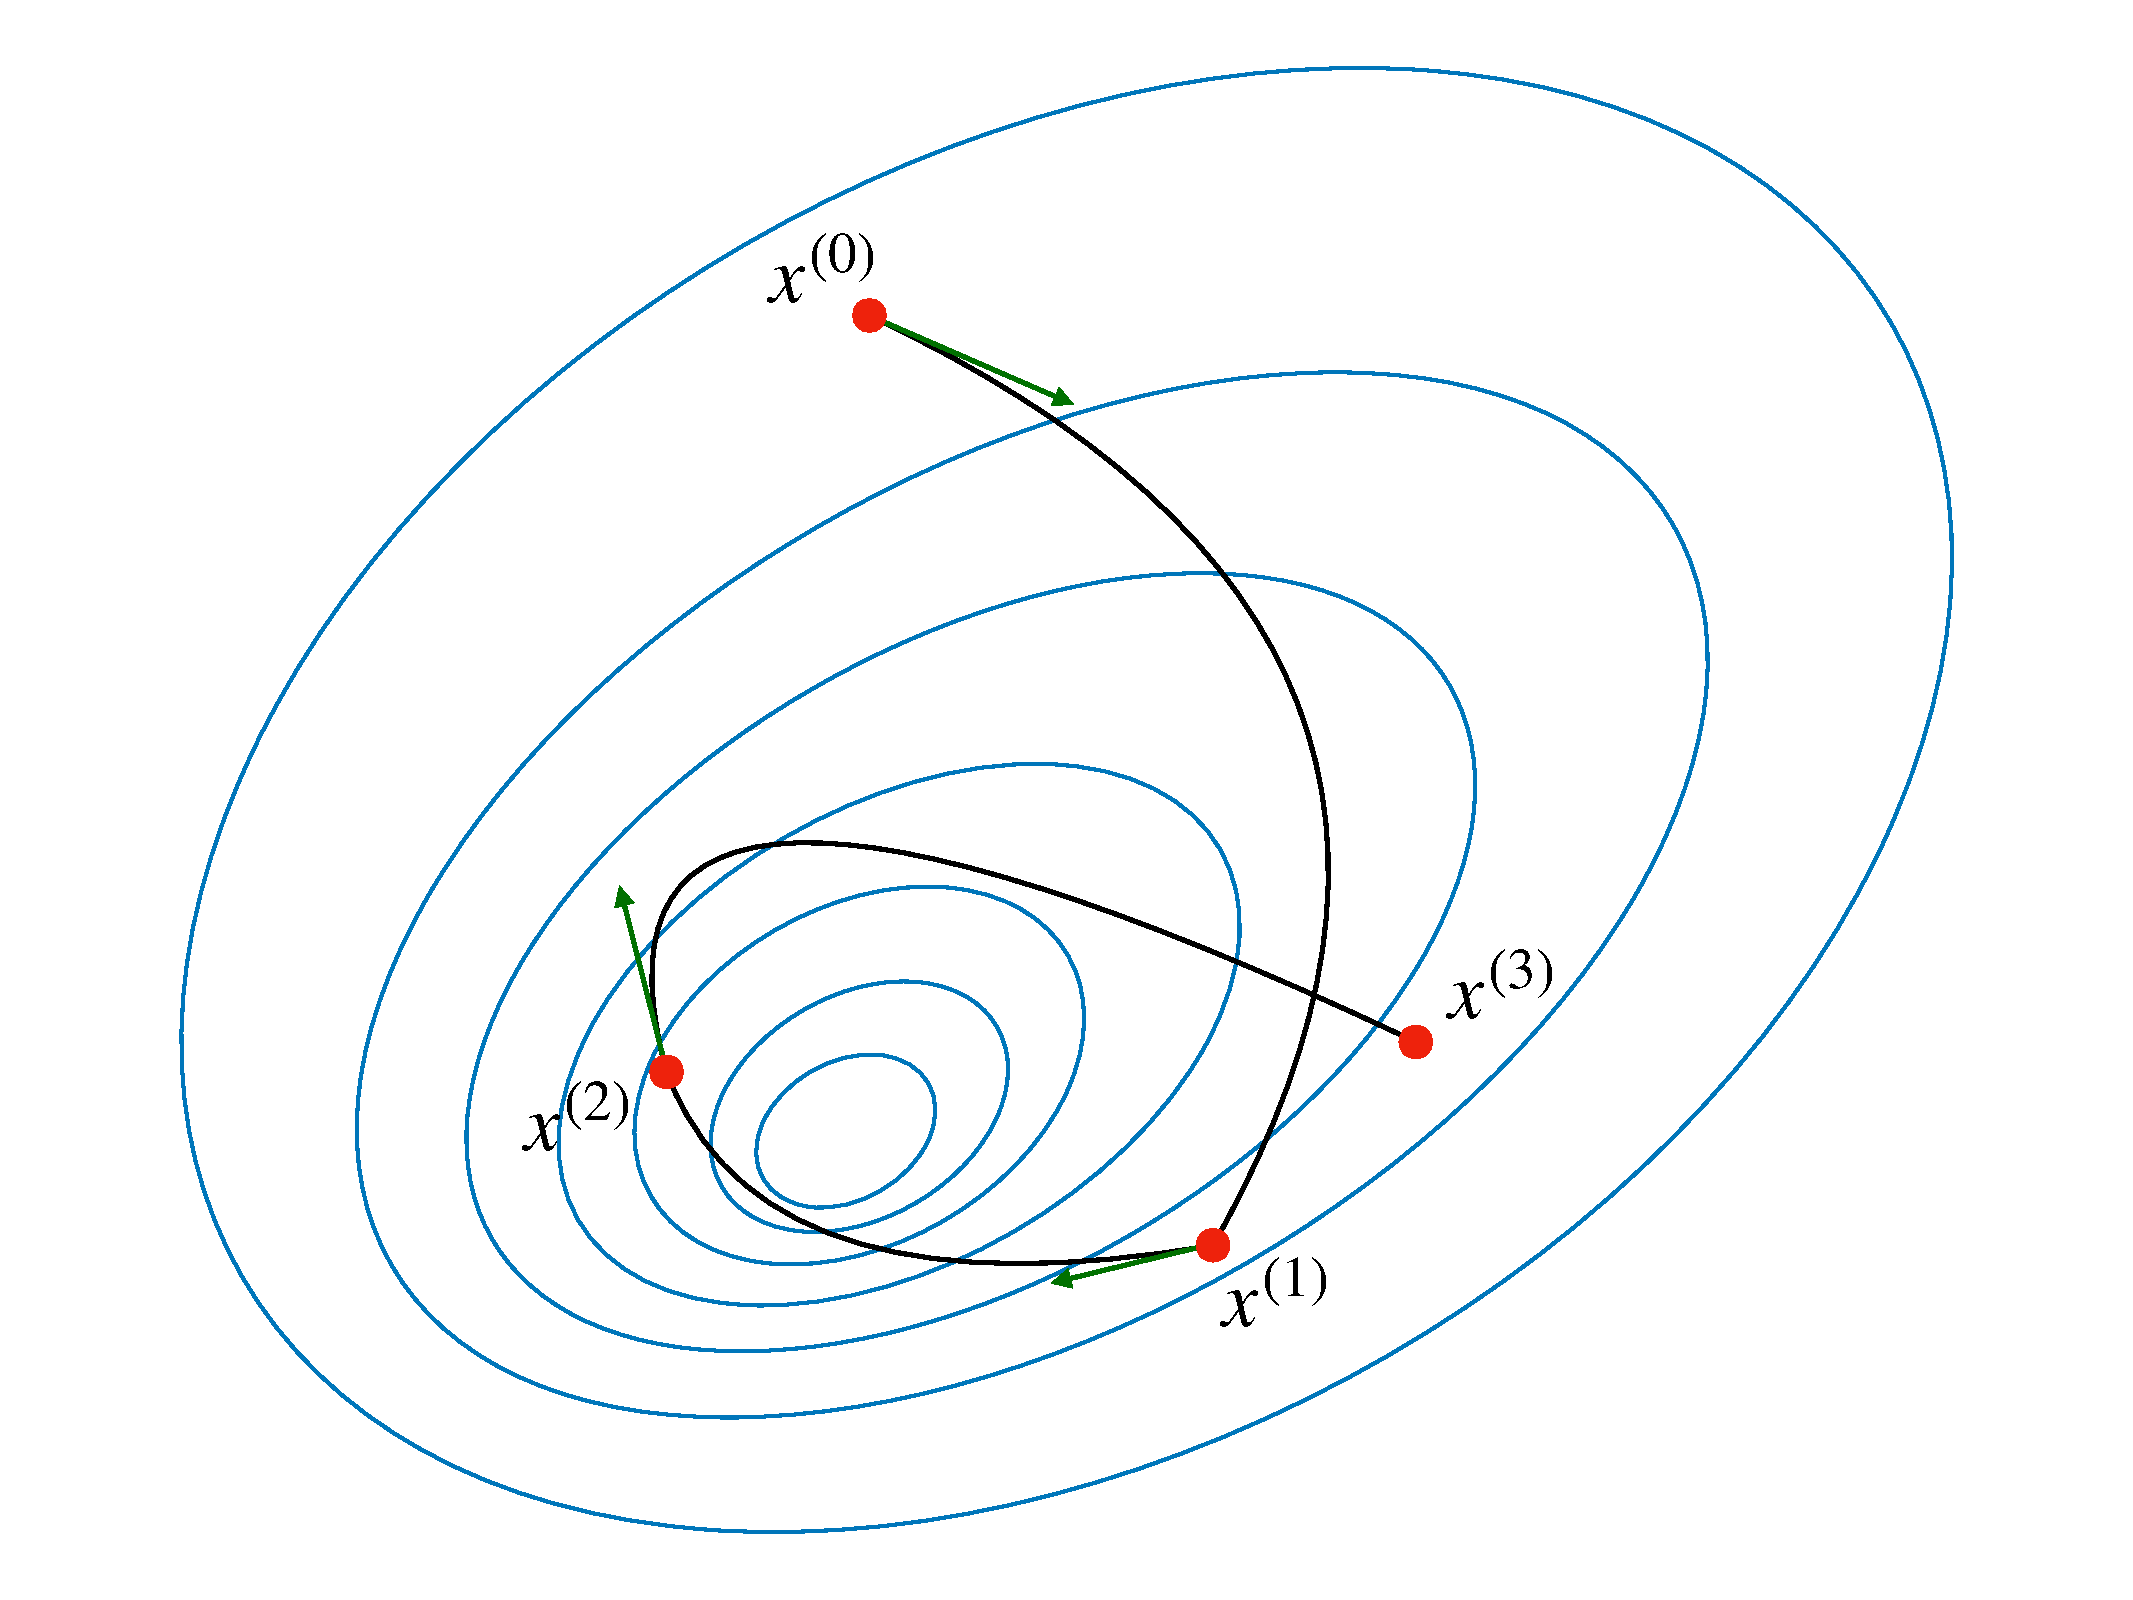
\includegraphics[width=0.7\textwidth]{../assets/887/fig}
    \end{center}
    \caption{A trajectory of Hamiltonian Monte Carlo}
    \label{fig:HMC}
\end{figure}


In our analysis, we first consider {\em ideal} HMC where in every step we have the exact solution to the ODE \eqref{eq:ODE_system} and neglect the numerical error from solving the ODEs or integration ($\delta = 0$). 

\subsection{Preliminaries}\label{sec:pre}
We recall
some  %
standard definitions here. Let $f:\R^d \to \R$ be a continuously differentiable function. 
%
For a positive real number $\mu$ we say that  %
$f$ is $\mu$-strongly convex if for all $x,y\in \R^d$, 
\[
f(y) \ge f(x) + \ip{\grad f(x)}{y-x} + \frac{\mu}{2} \norm{y-x}^2.
\]
We say
that  %
$f$ is $L$-smooth if $\grad f$ is $L$-Lipschitz, %
%
\ie, for all $x,y \in \R^d$,
\[
\norm{\grad f(x) - \grad f(y)} \le L \norm{x-y}.
\]
If $f$ is $\mu$-strongly convex and $L$-smooth, then the condition number of $f$ is $\kappa = L/\mu$.
When $f$ is a twice differentiable function, $f$ is $\mu$-strongly convex if and only if $\grad^2 f(x) \succeq \mu I$ for all $x\in \R^d$, where $\grad^2 f(x)$ denotes the Hessian matrix of $f$ at $x$ and $I$ is the identity matrix; similarly, $f$ is $L$-smooth if and only if $\grad^2 f(x) \preceq LI$ for all $x \in \R^d$. 

%
%
%
Consider a discrete-time \emph{reversible} Markov chain $\mathcal{M}$ on $\R^d$ with stationary distribution $\pi$. 
Let
\[
L_2(\pi) = \left\{ f: \R^d \to \R \,\middle|\, \int_{\R^d} f(x)^2 \pi(\dif x) < \infty \right\}
\]
be the Hilbert space with inner product
\[
\ip{f}{g} = \int_{\R^d} f(x) g(x) \pi(\dif x)
\]
for $f,g \in L_2(\pi)$. 
Denote by $P$ the transition kernel of $\mathcal{M}$. 
We can view $P$ as a self-adjoint operator from $L_2(\pi)$ to itself: for $f\in L_2(\pi)$, 
\[
(Pf) (x) = \int_{\R^d} f(y)P(x,\dif y).
\]
%
Let $L_2^0(\pi) = \{ f\in L_2(\pi): \int_{\R^d} f(x) \pi(\dif x) = 0 \}$ be a closed subspace of $L_2(\pi)$. The (absolute) \emph{spectral gap} of $P$ is defined to be
\[
\gamma(P) = 1 - \sup_{f\in L_2^0(\pi)}\frac{\norm{Pf}}{\norm{f}} = 1 - \sup_{\substack{f\in L_2^0(\pi)\\ \norm{f} = 1}} |\ip{Pf}{f}|.
\]
The relaxation time of $P$ is 
\[
\Trel(P) = \frac{1}{\gamma(P)}.
\]

Let $\nu_1,\nu_2$ be two distributions on $\R^d$ with finite $p$'th moments where $p \ge 1$. 
The $p$-Wasserstein distance between $\nu_1$ and $\nu_2$ is defined as
\[
W_p(\nu_1,\nu_2) = \left( \inf_{(X,Y) \in \mathcal{C}(\nu_1,\nu_2)} \Exp\left[ \norm{X-Y}^p \right] \right)^{1/p},
\]
where $\mathcal{C}(\nu_1,\nu_2)$ is the set of all couplings of $\nu_1$ and $\nu_2$. 
The Ricci curvature of $P$ is defined as
\[
\mathrm{Ric}(P) = 1 - \sup_{x,y \in \R^d, x \neq y} \frac{W_1(P(x, \cdot), P(y, \cdot))}{\norm{x-y}}. 
\]
It is known that $\gamma(P) \ge \mathrm{Ric}(P)$ (see \cite[Proposition 29]{O09}), which provides an effective way to bound the spectral gap through coupling arguments. 
We refer to \cite{O09} for more backgrounds on the Ricci curvature. 
	
	

\subsection{Related work}
Various versions of Langevin dynamics have been studied in many recent papers, see \cite{D17,DK19, ZLC17,RRT17, DRD18,CCBJ, CCABJ18,CFMBJ18, DCWY18,W18, VW19,MCCFBJ19}. 
The convergence rate of HMC %
has also been   %
studied recently in \cite{LSV18,LV18,MS17, MS19,MV18,SRH14}. 
%
The first bound %
in  %
our setting was obtained by Mangoubi and Smith \cite{MS17}, who gave an $O(\kappa^2)$ bound on the convergence rate of ideal HMC. 

\begin{theorem}[{\cite[Theorem 1]{MS17}}]
	Let $f:\R^d \to\R$ be a twice differentiable function such that $\mu I \preceq \grad^2 f(x) \preceq L I$ for all $x\in\R^d$. 
	Then the relaxation time of ideal HMC for sampling from the density $\propto \eee^{-f}$ with step-size $T = \sqrt{\mu}/(2\sqrt{2} L)$ is $O(\kappa^{2})$.  
\end{theorem}


This was improved by \cite{LSV18}, which showed a bound of $O(\kappa^{1.5})$. 
They also gave an algorithm with nearly optimal running time for solving the ODE that arises in the implementation of HMC.  

\begin{theorem}[{\cite[Lemma 1.8]{LSV18}}]
	Let $f:\R^d \to\R$ be a twice differentiable function such that $\mu I \preceq \grad^2 f(x) \preceq L I$ for all $x\in\R^d$. 
	Then the relaxation time of ideal HMC for sampling from the density $\propto \eee^{-f}$ with step-size $T = \mu^{1/4}/(2L^{3/4})$ is $O(\kappa^{1.5})$.  
	%
\end{theorem}


Both papers suggest that the correct bound is linear in $\kappa$. 
It is mentioned in \cite{MS17} that linear dependency is the best one can expect. 
Meanwhile, \cite{LSV18} shows that there {\em exists} a choice of step-sizes (time for running the ODE), which depends on $f$, the current position, and the random initial velocity, that achieves a linear convergence rate (Lemma 1.8, second part); however it was far from clear how to determine these step-sizes algorithmically.  

Other papers focus on various aspects and use stronger assumptions (\eg, bounds on higher-order gradients) to get better bounds on the overall convergence time or the number of gradient evaluations in some ranges of parameters. For example, \cite{MV18} shows that the dependence on dimension for the number of gradient evaluations can be as low as $d^{1/4}$ with suitable regularity assumptions (and higher dependence on the condition number). We note also that sampling logconcave functions is a polynomial-time solvable problem, without the assumptions of strong convexity or gradient Lipschitzness, and even when the function $\eee^{-f}$ is given only by an oracle with no access to gradients \cite{AK91, LV06}. The Riemannian version of HMC provides a faster polynomial-time algorithm for uniformly sampling polytopes \cite{LV18}. However, the dependence on the dimension is significantly higher for these algorithms, both for the contraction rate and the time per step. 

After the %
conference version~\cite{conf-version}   %
of our paper, %
several articles appeared  %
%
on sampling from logconcave densities. 
For example, \cite{CLW19, DRK19, MMWBJ19, SL19, W19} study the 
Langevin dynamics and its variants, and \cite{CDWY19, LST20} 
study Metropolized HMC. 
%
%
%
Shen and Lee~\cite{SL19} propose the  %
Randomized Midpoint Method to discretize the underdamped Langevin diffusion; 
their algorithm achieves smaller number of total gradient calls
%
%
%
$N = \tilde{O}( \kappa^{7/6} d^{1/6} \eps^{-1/3}
 + \kappa d^{1/3} \eps^{-2/3} )$ 
and less running time compared to our HMC method. 
%
%
%
%

\subsection{Results}
In this paper, we show that the relaxation time of ideal HMC is $\Theta(\kappa)$ for strongly logconcave functions with Lipschitz gradient.  
\begin{theorem}\label{thm:rel_upper}
	Suppose that $f$ is $\mu$-strongly convex and $L$-smooth. Then the relaxation time (inverse of spectral gap) of ideal HMC for sampling from the density $\propto \eee^{-f}$ with step-size $T = 1/(2\sqrt{L})$ is $O(\kappa)$, 
	%
	%
	%
	where $\kappa = L/\mu$ is the condition number. 
\end{theorem}

We remark that the only assumption we made about $f$ is strong convexity and
%
smoothness. (In particular,  %
we do not require that $f$ is twice differentiable, which is assumed in both \cite{LSV18} and \cite{MS17}.)   %

We also establish a matching lower bound on the relaxation time of ideal HMC, implying the tightness of \expref{Theorem}{thm:rel_upper}. 
\begin{theorem}\label{thm:rel_lower}
	For any $L \ge \mu > 0$ and $T>0$, there exists a $\mu$-strongly convex and $L$-smooth function~$f$, such that the relaxation time of ideal HMC for sampling from the density $\propto \eee^{-f}$ with step-size $T$ is $\Omega(\kappa)$, where $\kappa = L/\mu$ is the condition number. 
\end{theorem}

Using the ODE solver from \cite{LSV18} with nearly optimal running time, we obtain the following convergence rate in 2-Wasserstein distance for the HMC algorithm. 
%
\begin{theorem}
	\label{thm:mixing}
	%
	%
	%
	%
	%
	Let $\pi \propto \eee^{-f}$ be the target distribution, and let $\pi_{\textsc{hmc}}$ be the distribution of the output of HMC with starting point $x^{(0)} = \arg\min_x f(x)$, step-size $T = 1/(16000\sqrt{L})$, and 
	ODE error tolerance $\delta = \sqrt{\mu}T^2 \eps/16$.
	For any $0<\eps<\sqrt{d}$, if we run HMC for $N = O\left( \kappa \log(d/\eps) \right)$ steps where $\kappa = L/\mu$, then we have 
	\begin{equation}
	%
	W_2(\pi_{\textsc{hmc}},\pi) \le \frac{\eps}{\sqrt{\mu}}.
	\end{equation}
	Each step takes $O\left( \sqrt{\kappa}d^{3/2}\eps^{-1} \log(\kappa d/\eps) \right)$ time and $O\big( \sqrt{\kappa d}\eps^{-1} \log(\kappa d/\eps) \big)$ evaluations of $\grad f$, amortized over all steps.
\end{theorem}
We note that since our new convergence rate allows larger steps, the ODE solver is run for a longer time step. 
One interesting open problem is to find a matching lower bound for HMC with respect to the 2-Wasserstein distance. 

The comparison of convergence rates, running times and numbers of gradient evaluations is summarized in the following table with polylog factors omitted. 

\begin{center}
{\renewcommand{\arraystretch}{1.3}%
	\begin{tabular}{c|c|c|c}
	\hline
	reference & convergence rate & \# gradients & total time\\
	\hline
\cite{MS17} & $\kappa^2$ & $\kappa^{6.5} d^{\,0.5}$  & $\kappa^{6.5} d^{1.5}$ \\
\cite{LSV18} & $\kappa^{1.5}$ & $\kappa^{1.75} d^{\,0.5}$ &  $\kappa^{1.75} d^{1.5}$ \\
this paper & $\kappa$ & $\kappa^{1.5} d^{\,0.5}$ & $\kappa^{1.5} d^{1.5}$\\
\hline
\end{tabular}
	}
\end{center}

Finally, we remark that \expref{Theorem}{thm:rel_lower} also implies an $\Omega(\kappa)$ computational lower bound for HMC in terms of the number of gradient queries. 
This differs from \cite{SL19} by a factor of $\tilde{O}(\kappa^{1/6})$. 
As pointed out by one of the referees, 
a comparison with optimization literature seems to suggest that the optimal number of gradient queries that can be achieved by any gradient-based MCMC algorithm should scale as $\sqrt{\kappa}$. 
This corroborates with the fine analysis in \cite{CLW19} that the convergence rate of continuous underdamped Langevin dynamics is $O(\sqrt{m})$ where $m$ is the Poincar\'{e} constant of the measure, 
suggesting that an ideal discretization of underdamped Langevin dynamics with step-size $O(\sqrt{1/L})$ might be able to achieve $O(\sqrt{\kappa})$ convergence. 
In this sense, HMC probably cannot achieve the optimal convergence.



\section{Convergence of ideal HMC}
In this section we show that the spectral gap of ideal HMC is $\Omega(1/\kappa)$, and thus prove \expref{Theorem}{thm:rel_upper}. 
We first show a contraction bound for ideal HMC, which roughly says that the distance of two points is shrinking after one step of ideal HMC. 

\begin{lemma}[Contraction bound]
	\label{lem:HMC_contraction}
	Suppose that $f$ is $\mu$-strongly convex and $L$-smooth. Let $x(t)$ and $y(t)$ be the solution to \eqref{eq:ODE_system} with initial positions $x(0)$, $y(0)$ and initial velocities $x'(0) = y'(0)$. Then for $0\le t \le 1/(2\sqrt{L})$ we have
	\begin{equation}
	%
	\norm{x(t) - y(t)}^2 \le \left( 1 - \frac{\mu}{4} t^2 \right) \norm{x(0) - y(0)}^2.
	\end{equation}
	In particular, by setting $t = T = 1/(c\sqrt{L})$ for some constant $c \ge 2$ we get
	\begin{equation}
	%
	\norm{x(T) - y(T)}^2 \le \left( 1 - \frac{1}{4c^2 \kappa} \right) \norm{x(0) - y(0)}^2
	\end{equation}
	where $\kappa = L/\mu$.
\end{lemma}


\begin{proof}%
	Consider the two ODEs for HMC:
	\[
	\left\{\,
	\begin{aligned}
	x'(t) &= u(t);\\
	u'(t) &= -\grad f(x(t)).
	\end{aligned}
	\right.
	\qquad\text{and}\qquad
	\left\{\,
	\begin{aligned}
	y'(t) &= v(t);\\
	v'(t) &= -\grad f(y(t)).
	\end{aligned}
	\right.
	\]
	with initial points $x(0), y(0)$ and initial velocities $u(0) = v(0)$. 
	%
	We will show that
	\[
	\norm{x(t)-y(t)}^2 \leq \left( 1 - \frac{\mu}{4} t^2 \right) \norm{x(0) - y(0)}^2
	\]
	for all $0 \le t \le 1/(2\sqrt{L})$. 
	
	Consider the derivative of $\frac{1}{2} \norm{x(t)-y(t)}^2$:
	\begin{equation}\label{eqn:deri_x-y}
	\frac{\dif}{\dif t} \left( \frac{1}{2} \norm{x(t)-y(t)}^2 \right) = 
	%
	\ip{x'(t)-y'(t)}{x(t)-y(t)} = \ip{u(t)-v(t)}{x(t)-y(t)}.
	\end{equation}
	Taking derivative on both sides, we get
	\begin{align}
	\frac{\dif^2}{\dif t^2} \left( \frac{1}{2} \norm{x(t)-y(t)}^2 \right) 
		%
  &= \ip{u'(t)-v'(t)}{x(t)-y(t)} + \ip{u(t)-v(t)}{x'(t)-y'(t)} \nonumber\\
  &= - \ip{\grad f(x(t)) - \grad f(y(t))}{x(t)-y(t)} + \norm{u(t)-v(t)}^2 \nonumber\\ 
  &= - \rho(t) \norm{x(t)-y(t)}^2 + \norm{u(t)-v(t)}^2, \label{eqn:deri2_x-y}
	\end{align}
where we define
	\[
	\rho(t) = \frac{\ip{\grad f(x(t)) - \grad f(y(t))}{x(t)-y(t)}}{\norm{x(t)-y(t)}^2}.
	\]
	Since $f$ is $\mu$-strongly convex and $L$-smooth, we have $\mu \le \rho(t) \le L$ for all $t\geq 0$.
	
We will %
give an upper bound on  %
the term $- \rho(t)\norm{x(t)-y(t)}^2 + \norm{u(t)-v(t)}^2$, while keeping its dependency on $\rho(t)$. To lower bound $\norm{x(t)-y(t)}^2$, we use the following crude bound.
	\begin{claim}[Crude bound]
		\label{claim:crude-bound}
		For all $0 \le t \le 1/(2\sqrt{L})$ we have
		\begin{equation}\label{eqn:crude_bound}
		\frac{1}{2} \norm{x(0) - y(0)}^2 \le \norm{x(t)-y(t)}^2 \le 2 \norm{x(0) - y(0)}^2.
		\end{equation}
	\end{claim}
	\noindent
	The proof of this claim is postponed to \expref{Section}{subsec:proof_claim}. 
	
	Next we derive an upper bound on $\norm{u(t)-v(t)}^2$. 
	By taking the derivative of $\frac{1}{2} \norm{u(t)-v(t)}^2$, we get
	\begin{align*}
		\norm{u(t)-v(t)} \left( \frac{\dif}{\dif t} \norm{u(t)-v(t)} \right) 
		&= \frac{\dif}{\dif t} \left( \frac{1}{2} \norm{u(t)-v(t)}^2 \right)\\ 
		&= \ip{u'(t)-v'(t)}{u(t)-v(t)}\\ 
		&= - \ip{\grad f(x(t)) - \grad f(y(t))}{u(t)-v(t)}.
	\end{align*}
Thus, its absolute value is 
%
not greater than  %
	\[
	\left| \frac{\dif}{\dif t} \norm{u(t)-v(t)} \right| = \frac{\left| - \ip{\grad f(x(t)) - \grad f(y(t))}{u(t)-v(t)} \right|}{\norm{u(t)-v(t)}} \le \norm{\grad f(x(t)) - \grad f(y(t))}.
	\]
	Since $f$ is $L$-smooth and convex, it holds that 
	\[
	\norm{\grad f(x(t)) - \grad f(y(t))}^2 \le L \ip{\grad f(x(t)) - \grad f(y(t))}{x(t)-y(t)}; 
	\] 
	see, \eg, \cite[Lemma 4]{Zhou18} for a proof. Hence, we obtain 
	\[
	\norm{\grad f(x(t)) - \grad f(y(t))}^2 
	%
	\le L\rho(t) \norm{x(t)-y(t)}^2 \le 2L\rho(t) \norm{x(0)-y(0)}^2,
	\]
	where the last inequality follows from the crude bound \eqref{eqn:crude_bound}. 
	%
	%
	%
	%
	%
	%
Then, using the fact that $u(0)=v(0)$ and the Cauchy--Schwarz inequality, we can upper bound $\norm{u(t)-v(t)}^2$ by
	\begin{align*}
		\norm{u(t)-v(t)}^2 
		&\le \left( \int_{0}^t \left| \frac{\dif}{\dif s} \norm{u(s)-v(s)} \right| \dif s \right)^2\\ 
		&\le \left( \int_{0}^t \sqrt{2L\rho(s)} \norm{x(0)-y(0)} \dif s \right)^2\\ 
		&\le 2L t \left( \int_{0}^t \rho(s) \,\dif s \right) \norm{x(0)-y(0)}^2. 
	\end{align*}
	Define the function
	\[
	P(t) = \int_{0}^t \rho(s) \,\dif s,
	\]
	so $P(t)$ is nonnegative and monotone increasing, with $P(0) = 0$. Also we have $\mu t \le P(t) \le Lt$ for all $t\geq 0$. Then, 
	\begin{equation}\label{eqn:bound_u-v}
	\norm{u(t)-v(t)}^2 \le 2Lt P(t) \norm{x(0)-y(0)}^2.
	\end{equation}
	
	Plugging \eqref{eqn:crude_bound} and \eqref{eqn:bound_u-v} into \eqref{eqn:deri2_x-y}, we deduce that
	\begin{equation*}
		\frac{\dif^2}{\dif t^2} \left( \frac{1}{2} \norm{x(t)-y(t)}^2 \right) 
		%
		\le - \rho(t) \left( \frac{1}{2} \norm{x(0) - y(0)}^2 \right) + 2Lt P(t) \norm{x(0)-y(0)}^2. 
	\end{equation*}
	If we define
	\[
	\alpha(t) = \frac{1}{2} \norm{x(t)-y(t)}^2, 
	\]
	%
	then we have 
	\[
	\alpha''(t) \le - \alpha(0) \big( \rho(t)  - 4L t P(t) \big).
	\]
	Integrating both sides and using $\alpha'(0) = 0$, we obtain
	\begin{align*}
		\alpha'(t) &= \int_{0}^t \alpha''(s) \dif s\\ 
		&\le - \alpha(0) \left( \int_{0}^t \rho(s) \dif s - 4L \int_{0}^t sP(s) \dif s \right)\\ 
		&\le - \alpha(0) \left( P(t) - 4L P(t) \int_{0}^t s \dif s \right)\\ 
		&= - \alpha(0) P(t) \left( 1 - 2Lt^2 \right), 
	\end{align*}
	where the second inequality is due to the monotonicity of $P(s)$. 
	Since for all $0\le t\le 1/(2\sqrt{L})$ we have $P(t) \ge \mu t$ and $1-2Lt^2 \ge 1/2$, we deduce that
	\[
	\alpha'(t) \le - \alpha(0) \frac{\mu}{2} t.
	\]
	Finally, one more integration yields
	\[
	\alpha(t) = \alpha(0) + \int_{0}^t \alpha'(s) \dif s \le \alpha(0) \left( 1 - \frac{\mu}{4} t^2 \right), 
	\]
	and the theorem follows.
\end{proof}

\begin{proof}[Proof of \expref{Theorem}{thm:rel_upper}]
	%
	%
	%
	Recall from \expref{Section}{sec:pre} that the Ricci curvature of a Markov chain $P$ is defined to be 
	$1 - \sup_{x\neq y} W_1(P(x, \cdot), P(y, \cdot)) / \norm{x-y}$ where $W_1$ is the $1$-Wasserstein distance. 
	Then, \expref{Lemma}{lem:HMC_contraction} immediately implies that for any constant $c\ge 2$, the Ricci curvature of ideal HMC with step-size $T=1/(c\sqrt{L})$ is at least $1/(8c^2\kappa)$. 
	%
	It follows from \cite[Proposition 29]{O09} that the spectral gap of ideal HMC is at least $1/(8c^2\kappa)$. Hence, the relaxation time is
%
at most   %
$8c^2\kappa = O(\kappa)$.
\end{proof}


\subsection{Proof of \expref{Claim}{claim:crude-bound}}
\label{subsec:proof_claim}
%
We present the proof of \expref{Claim}{claim:crude-bound} in this section. We remark that a similar crude bound was established in \cite{LSV18} for general matrix ODEs. Here we prove the crude bound specifically for the Hamiltonian ODE, but without assuming that $f$ is twice differentiable.
\begin{proof}[Proof of \expref{Claim}{claim:crude-bound}]
	We first derive a crude upper bound on $\norm{u(t)-v(t)}$. Since $f$ is $L$-smooth, we have 
	\begin{align*}
		\frac{\dif}{\dif t} \norm{u(t)-v(t)} 
		&= \frac{- \ip{\grad f(x(t)) - \grad f(y(t))}{u(t)-v(t)}}{\norm{u(t)-v(t)}}\\
		&\le \norm{\grad f(x(t)) - \grad f(y(t))} 
		\le L \norm{x(t)-y(t)}.
	\end{align*}
	Then from $u(0) = v(0)$ we get
	\[
	\norm{u(t)-v(t)} = \int_{0}^t \left( \frac{\dif}{\dif s} \norm{u(s)-v(s)} \right) \dif s \le L \int_{0}^t \norm{x(s)-y(s)} \dif s.
	\]
	
	To obtain the upper bound for $\norm{x(t)-y(t)}$, we first bound its derivative by
	\begin{equation}\label{eqn:abs_deri_x-y}
	\left| \frac{\dif}{\dif t} \norm{x(t)-y(t)} \right| = \frac{\left| \ip{u(t)-v(t)}{x(t)-y(t)} \right|}{\norm{x(t)-y(t)}} \le \norm{u(t)-v(t)} \le L \int_{0}^t \norm{x(s)-y(s)} \dif s.
	\end{equation}
	Therefore, we have
	\begin{align*}
		\norm{x(t)-y(t)} &= \norm{x(0) - y(0)} + \int_{0}^t \left( \frac{\dif}{\dif s} \norm{x(s)-y(s)} \right) \dif s\\ 
		&\le \norm{x(0) - y(0)} + L \int_{0}^t \int_{0}^s \norm{x(r)-y(r)} \dif r \dif s\\
		&= \norm{x(0) - y(0)} + L \int_{0}^t (t-s) \norm{x(s)-y(s)} \dif s.
	\end{align*}
	%
	Then, applying a Gr\"{o}nwall-type inequality from \cite[Lemma A.5]{LSV18}, we deduce that
	\begin{equation}\label{eqn:upper_norm_x-y}
	\norm{x(t)-y(t)} \le \norm{x(0) - y(0)} \cosh\left( \sqrt{L}t \right) \le \sqrt{2} \norm{x(0) - y(0)},
	\end{equation}
	where we also use the fact that $\cosh(\sqrt{L} t) \leq \cosh(1/2) \le \sqrt{2}$.
	
	Next, we deduce from \eqref{eqn:abs_deri_x-y} and \eqref{eqn:upper_norm_x-y} that
	\begin{align*}
		\frac{\dif}{\dif t} \norm{x(t)-y(t)} 
		%
		%
		&\ge - L \int_{0}^t \norm{x(s)-y(s)} \dif s\\ 
		&\ge - L \norm{x(0) - y(0)} \int_{0}^t  \cosh\left( \sqrt{L}s \right) \dif s\\ 
		&= - \sqrt{L} \norm{x(0) - y(0)} \sinh\left( \sqrt{L} t \right).
	\end{align*}
	Thus, we obtain
	\begin{align*}
		\norm{x(t)-y(t)} &= \norm{x(0) - y(0)} + \int_{0}^t \left( \frac{\dif}{\dif s} \norm{x(s)-y(s)} \right) \dif s\\ 
		&\ge \norm{x(0) - y(0)} - \sqrt{L} \norm{x(0) - y(0)} \int_{0}^t \sinh\left( \sqrt{L} s \right) \dif s\\
		&= \norm{x(0) - y(0)} \left( 2 - \cosh\left( \sqrt{L} t \right) \right) \ge \frac{1}{\sqrt{2}} \norm{x(0) - y(0)},
	\end{align*}
	where we use $2 - \cosh(\sqrt{L} t) \ge 2- \cosh(1/2) \ge 1/\sqrt{2}$.
\end{proof}



\section{Lower bound for ideal HMC}
In this section, we show that the relaxation time of ideal HMC can be $\Theta(\kappa)$ for some $\mu$-strongly convex and $L$-smooth function for any step-size $T$, and thus prove \expref{Theorem}{thm:rel_lower}. 

Consider the following one-dimensional quadratic function:
\begin{equation}
%
f(x) = \frac{x^2}{2 \sigma^2},
\end{equation}
where $1/\sqrt{L} \le \sigma \le 1/\sqrt{\mu}$. 
Thus, $f$ is $\mu$-strongly convex and $L$-smooth. The probability density $\nu$ proportional to $\eee^{-f}$ is the Gaussian distribution: for $x\in \R$, 
\begin{equation}
%
\nu(x) = \frac{1}{\sqrt{2\pi} \sigma} \exp\left( - \frac{x^2}{2\sigma^2} \right).
\end{equation}
The following lemma shows that, for certain choice of $\sigma$,
ideal HMC for the Gaussian distribution $\nu$ can have relaxation time $\Omega(\kappa)$. 
\expref{Theorem}{thm:rel_lower} then follows immediately.


\begin{lemma}
	For any $T > 0$ there exists $1/\sqrt{L} \le \sigma \le 1/\sqrt{\mu}$ such that the relaxation time of ideal HMC for sampling from $\nu$ with step-size $T$ is at least $\kappa/(8\pi^2)$.
\end{lemma}
%

\begin{proof}
	The Hamiltonian curve for $f$ is given by the ODE
	\[
	x''(t) = - f'(x(t)) = -\frac{x(t)}{\sigma^2}
	\]
	with initial position $x(0) \in \R$ and initial velocity $x'(0)$ drawn from the standard Gaussian $N(0,1)$. 
	%
%
%
%
%
	%
	Solving the ODE and plugging in the step-size $t=T$, we get
	\[
	x(T) = x(0) \cos(T/\sigma) + v(0) \sigma \sin(T/\sigma).
	\]
	
	Consider first the case that $T > 4\pi/\sqrt{L}$. 
	We may assume that $L \ge 4\mu$ (\ie, $\kappa \ge 4$), since otherwise the lemma trivially holds. 
	Pick a positive integer $k$ such that
	\[
	\frac{T\sqrt{\mu}}{2\pi} \le k \le \frac{T\sqrt{L}}{2\pi}.
	\]
	Note that such $k$ exists as
	\[
	\frac{T\sqrt{L}}{2\pi} - \frac{T\sqrt{\mu}}{2\pi} \ge \frac{T\sqrt{L}}{4\pi} > 1.
	\]
	We then choose
	$\sigma = T/(2k\pi)$, 
	which satisfies $1/\sqrt{L} \le \sigma \le 1/\sqrt{\mu}$. 
	Observe that for such a choice HMC becomes degenerate: we have $x(T) = x(0)$, meaning that the chain does not move at all. 
	Thus, in this extremal case the relaxation time becomes infinity and the lemma holds.
	
	Next we consider the case that $T \le 4\pi/\sqrt{L}$.
	We shall pick $\sigma = 1/\sqrt{\mu}$. 
	Let $P$ denote the transition kernel of ideal HMC. 
	%
	Then for $x,y\in\R$ we have
	\[
	P(x,y) = \frac{1}{\sqrt{2\pi} \sigma \sin(T/\sigma)} \exp\left( - \frac{\left( y - x\cos(T/\sigma) \right)^2}{2\sigma^2 \sin^2(T/\sigma)} \right).
	\] 
	Namely, given the current position $x$, the next position $y$ is from a normal distribution with mean $x\cos(T/\sigma)$ and variance $\sigma^2 \sin^2(T/\sigma)$. 
	Denote the spectral gap of $P$ by $\gamma$. 
	Let $h(x) = x$ and note that $h\in L^0_2(\nu)$. Using the properties of spectral gaps, we deduce that
	\[
	\gamma 
	= 1 - \sup_{f\in L_2^0(\nu)} \frac{|\ip{P f}{f}|}{\norm{f}^2}
	\le 1 - \frac{|\ip{P h}{h}|}{\norm{h}^2}. 
	%
	%
	\]
	Since we have
	\[
	\norm{h}^2 = \int_{-\infty}^{\infty} \nu(x) h(x)^2 \dif x = \sigma^2
	\]
	and
	\[
	\ip{P h}{h} = \int_{-\infty}^{\infty} \nu(x) P(x,y) h(x) h(y) \dif x \dif y = \sigma^2 \cos(T/\sigma),
	\]
	%
	%
	%
	we then get 
	\[
	\gamma \le 1 - |\cos(T/\sigma)| 
	\le \frac{T^2}{2\sigma^2} \le 8\pi^2 \cdot \frac{\mu}{L}
	\]
	where the last inequality is due to our assumption $T \le 4\pi/\sqrt{L}$. 
	Hence, $\Trel = 1/\gamma \ge \kappa/(8\pi^2)$. 
	This completes the proof of the lemma. 
\end{proof}

%
%
%
%
%
%
%
%
%
%
%
%
%
%
%
%
%
%
%
%
%
%
%
%
%
%
%
%
%
%
%
%
%
%
%
%
%
%
%
%
%
%
%
%
%
%
%
%
%
%
%
%
%
%
%
%
%
%
%
%
%
%
%
%
%
%
%
%
%
%
%
%
%
%
%
%
%
%
%
%
%
%
%
%
%
%
%






\section{Convergence rate of discretized HMC}
In this section, we show how our improved contraction bound (\expref{Lemma}{lem:HMC_contraction}) implies that HMC returns a good enough sample after $\tilde{O}((\kappa d)^{1.5})$ steps. We will use the framework from \cite{LSV18} to establish \expref{Theorem}{thm:mixing}.

We first state the ODE solver from \cite{LSV18}, which solves an ODE in nearly optimal time when the solution to the ODE can be approximated by a piece-wise polynomial. We state here only for the special case of second order ODEs for the Hamiltonian system. We refer to \cite{LSV18} for general $k$th order ODEs.

\begin{theorem}[{\cite[Theorem 2.5]{LSV18}}]
	\label{thm:ODE_solver}
	Let $x(t)$ be the solution to the ODE
	\begin{equation}
	%
	x''(t) = -\grad f(x(t)), \quad x(0) = x_0, \quad x'(0) = v_0.
	\end{equation}
	where $x_0,v_0 \in \R^d$ and $0\le t\le T$. Suppose that the following conditions hold:
	\begin{enumerate}
		\item There exists a piece-wise polynomial $q(t)$ such that $q(t)$ is a polynomial of degree $D$ on each interval $[T_{j-1},T_j]$ where $0=T_0 < T_1 < \dots <T_m = T$, and for all $0\le t\le T$ we have
		\begin{equation}
		%
		\norm{q(t) - x''(t)} \le \frac{\delta}{T^2};
		\end{equation}
		\item $\{T_j\}_{j=1}^m$ and $D$ are given as input to the ODE solver;
		\item The function $f$ has a $L$-Lipschitz gradient; \ie, for all $x,y\in\R^d$,
		\begin{equation}
		%
		\norm{\grad f(x) - \grad f(y)} \le L \norm{x-y}.
		\end{equation}
	\end{enumerate}
	If $\sqrt{L} T \le 1/16000$, then the ODE solver can find a piece-wise polynomial $\tilde{x}(t)$ such that for all $0\le t\le T$,
	\begin{equation}
	%
	\norm{\tilde{x}(t) - x(t)} \le O(\delta).
	\end{equation}
	The ODE solver uses $O(m(D+1) \log(CT/\delta))$ evaluations of $\grad f$ and $O(dm (D+1)^2 \log(CT/\delta))$ time where
	\begin{equation}
	%
	C = O\left(\norm{v_0} + T\norm{\grad f(x_0)} \right).
	\end{equation}
\end{theorem}

The following lemma, which combines Theorem~3.2, Lemma 4.1 and Lemma 4.2 from \cite{LSV18}, establishes the conditions of \expref{Theorem}{thm:ODE_solver} in our setting. We remark that Lemmas 4.1 and 4.2 hold for all $T \le 1/(8\sqrt{L})$, and Theorem~3.2, though stated only for $T \le O(\mu^{1/4}/L^{3/4})$ in \cite{LSV18}, holds in fact for the whole region $T \le 1/(2\sqrt{L})$ where the contraction bound (\expref{Lemma}{lem:HMC_contraction}) is true. We omit these proofs here and refer the readers to \cite{LSV18} for more details.

\begin{lemma}\label{lem:ODE_prep}
	Let $f$ be a twice differentiable function such that $\mu I \preceq \grad^2 f(x) \preceq LI$ for all $x\in \R^d$. Choose the starting point $x^{(0)} = \arg\min_x f(x)$, step-size $T = 1/(16000\sqrt{L})$, and ODE error tolerance $\delta = \sqrt{\mu}T^2 \eps/16$ in the HMC algorithm. Let $\{x^{(k)}\}_{k=1}^N$ be the sequence of points we get from the HMC algorithm and $\{v_0^{(k)}\}_{k=1}^N$ be the sequence of random Gaussian vector we choose in each step. Let $\pi \propto \eee^{-f}$ be the target distribution and let $\pi_{\textsc{hmc}}$ be the distribution of $x^{(N)}$, \ie, the output of HMC. For any $0<\eps<\sqrt{d}$, if we run HMC for 
	\begin{equation}
	%
	N = O\left( \frac{\log(d/\eps)}{\mu T^2} \right) = O\left( \kappa \log(d/\eps) \right)
	\end{equation}
	steps where $\kappa = L/\mu$, then:
	\begin{enumerate}
		\item \emph{(\cite[Theorem 3.2]{LSV18})} We have that
		\begin{equation}
		%
		W_2(\pi_{\textsc{hmc}},\pi) \le \frac{\eps}{\sqrt{\mu}};
		\end{equation}
		\item \emph{(\cite[Lemma 4.1]{LSV18})} For each $k$, let $x_k(t)$ be the solution to the ODE \eqref{eq:ODE_Ham} in the $k$th step of HMC. Then there is a piece-wise constant function $q_k$ of $m_k$ pieces such that $\norm{q_k(t)-x_k''(t)} \le \delta/T^2$ for all $0\le t\le T$, where
		\begin{equation}
		%
		m_k = \frac{2LT^3}{\delta}\left( \norm{v_0^{(k-1)}} + T\norm{\grad f(x^{(k-1)})} \right);
		\end{equation}
		\item \emph{(\cite[Lemma 4.2]{LSV18})} We have that
		\begin{equation}
		%
		\frac{1}{N}\, \Exp\left[ \sum_{k=1}^{N} \norm{\grad f(x^{(k-1)})}^2 \right] \le O(Ld).
		%
		\end{equation}
	\end{enumerate}		
\end{lemma}


\begin{proof}[Proof of \expref{Theorem}{thm:mixing}]
	The convergence of HMC is guaranteed by part 1 of \expref{Lemma}{lem:ODE_prep}. In the $k$th step, the number of evaluations of $\grad f$ is $O(m_k \log (C_k \sqrt{\kappa}/\eps))$ by \expref{Theorem}{thm:ODE_solver} and part 2 of \expref{Lemma}{lem:ODE_prep}, where
	\[
	m_k = O\left( \frac{\sqrt{\kappa}}{\eps}\right) \left( \norm{v_0^{(k-1)}} + T\norm{\grad f(x^{(k-1)})}  \right) 
	\]
	and
	\[
	C_k = O\left( \norm{v_0^{(k-1)}} + T\norm{\grad f(x^{(k-1)})} \right).
	\]
Thus, the average number of evaluations of $\grad f$ per step is
%
not greater than  %
	\[
	\frac{1}{N}\, \Exp \left[ \sum_{k=1}^N O(m_k \log (C_k \sqrt{\kappa}/\eps)) \right] \le \frac{1}{N}\, \Exp \left[ \sum_{k=1}^N O(m_k \log m_k) \right]
	\le \frac{1}{N} \, O\left( \Exp \left[ M \log M \right] \right),
	\]
	where $M = \sum_{k=1}^N m_k$. Since each $v_0^{(k-1)}$ is sampled from the standard Gaussian distribution, we have $\Exp \Big[ \norm{v_0^{(k-1)}}^2 \Big] = d$. Thus, by the Cauchy--Schwarz inequality and part 3 of \expref{Lemma}{lem:ODE_prep}, we get
	\begin{align*}
		\Exp\left[ M^2 \right] \le N \sum_{k=1}^N \Exp\left[ m_k^2 \right] 
		&\le O\left( \frac{N\kappa}{\eps^2} \right) \sum_{k=1}^N \Exp\left[ \norm{v_0^{(k-1)}}^2 \right] + T^2 \Exp\left[ \norm{\grad f(x^{(k-1)})}^2 \right]\\ 
		&\le O\left( \frac{N^2\kappa d}{\eps^2} \right).
	\end{align*}
	We then deduce again from the Cauchy--Schwarz inequality that
	\[
	\left(\Exp[M \log M]\right)^2 \le \Exp\left[M^2\right] \cdot \Exp\left[\log^2 M\right] \le \Exp\left[ M^2 \right] \cdot \log^2\left( \Exp M \right) 
	\le \Exp[M^2] \cdot \log^2\left( \sqrt{\Exp\left[ M^2 \right]} \right), 
	%
	\]
	where the second inequality is due to Jensen's inequality and the fact that $\log^2(x)$ is concave when $x \geq 3$ (note that we can assume $M \ge 3$ by making $N \ge 3$). 
	Therefore, the number of evaluations of $\grad f$ per step, amortized over all steps, is 
	\[
	\frac{1}{N}\, O\left( \sqrt{\Exp[M^2]}  \log\left( \sqrt{\Exp\left[ M^2 \right]} \right) \right) \le O\left( \frac{\sqrt{\kappa d}}{\eps} \log\left( \frac{\kappa d}{\eps} \right) \right).
	\]
	Using a similar argument we have the bound for the expected running time per step. This completes the proof.
\end{proof}

\paragraph{Acknowledgments.} We are grateful to Yin Tat Lee and Andre Wibisono for helpful discussions. 
We also thank the anonymous referees for their valuable comments and suggestions. 













%% Theory of Computing
%% File: v018a009.bbl
%% Publication date: April 30, 2022
%% Authors: Zongchen Chen and Santosh S. Vempala
\newcommand{\prelim}{Preliminary version in\ }\newcommand{\prelims}{Preliminary
  versions in\ }
% Define empty bibhead if not already defined
\providecommand{\bibhead}[1]{}
% Define tocrefpdfbookmark if not already defined
\expandafter\ifx\csname pdfbookmark\endcsname\relax%
  \providecommand{\tocrefpdfbookmark}{}
\else\providecommand{\tocrefpdfbookmark}{%
   \hypertarget{tocreferences}{}%
   \pdfbookmark[1]{References}{tocreferences}}%
\fi

\tocrefpdfbookmark
\begin{thebibliography}{10}

\bibitem{AK91}\bibhead{AK91}
{\sc David Applegate and Ravi Kannan}: Sampling and integration of near
  log-concave functions.
\newblock In {\em Proc. 23rd STOC}, pp. 156--163. ACM Press, 1991.
\newblock [\epfmtdoi{10.1145/103418.103439}]

\bibitem{CLW19}\bibhead{CLW19}
{\sc Yu~Cao, Jianfeng Lu, and Lihan Wang}: On explicit ${L}^2$-convergence rate
  estimate for underdamped {L}angevin dynamics, 2019.
\newblock [\epfmt{arxiv}{1908.04746}]

\bibitem{CFMBJ18}\bibhead{CFMBJ18}
{\sc Niladri~S. Chatterji, Nicolas Flammarion, Yi-An Ma, Peter~L. Bartlett, and
  Michael~I. Jordan}: On the theory of variance reduction for stochastic
  gradient {M}onte {C}arlo.
\newblock In {\em Proc. 35th Internat. Conf. Artificial Intelligence and
  Statistics (ICML'18)}, pp. 80:764--773. MLR Press, 2018.
\newblock \href{http://proceedings.mlr.press/v80/chatterji18a.html}{PMLR}.
\newblock [\epfmt{arxiv}{1802.05431}]

\bibitem{CDWY19}\bibhead{CDWY19}
{\sc Yuansi Chen, Raaz Dwivedi, Martin~J. Wainwright, and Bin Yu}: Fast mixing
  of {M}etropolized {H}amiltonian {M}onte {C}arlo: {B}enefits of multi-step
  gradients.
\newblock {\em JMLR}, 21(92):1--72, 2019.
\newblock \href{https://jmlr.org/papers/v21/19-441.html}{JMLR}.
\newblock [\epfmt{arxiv}{1905.12247}]

\bibitem{conf-version}\bibhead{conf-version}
{\sc Zongchen Chen and Santosh~S. Vempala}: Optimal convergence rate of
  {H}amiltonian {M}onte {C}arlo for strongly logconcave distributions.
\newblock In {\em Proc. 23rd Internat. Conf. on Randomization and Computation
  (RANDOM'19)}, pp. 64:1--12. Schloss Dagstuhl--Leibniz-Zentrum fuer
  Informatik, 2019.
\newblock [\epfmtdoi{10.4230/LIPIcs.APPROX-RANDOM.2019.64},
  \epfmt{arxiv}{1905.02313}]

\bibitem{CCABJ18}\bibhead{CCABJ18}
{\sc Xiang Cheng, Niladri~S. Chatterji, Yasin Abbasi-Yadkori, Peter~L.
  Bartlett, and Michael~I. Jordan}: Sharp convergence rates for {L}angevin
  dynamics in the nonconvex setting, 2018.
\newblock [\epfmt{arxiv}{1805.01648}]

\bibitem{CCBJ}\bibhead{CCBJ}
{\sc Xiang Cheng, Niladri~S. Chatterji, Peter~L. Bartlett, and Michael~I.
  Jordan}: Underdamped {L}angevin {MCMC}: {A} non-asymptotic analysis.
\newblock In {\em Proc. 31st Ann. Conf. on Learning Theory (COLT'18)}, pp.
  75:1--24. MLR Press, 2018.
\newblock \href{https://proceedings.mlr.press/v75/cheng18a.html}{PMLR}.
\newblock [\epfmt{arxiv}{1707.03663}]

\bibitem{D17}\bibhead{D17}
{\sc Arnak~S. Dalalyan}: Theoretical guarantees for approximate sampling from
  smooth and log-concave densities.
\newblock {\em J. Royal Statistical Soc. Ser. B}, 79(3):651--676, 2017.
\newblock [\epfmtdoi{10.1111/rssb.12183}, \epfmt{arxiv}{1412.7392}]

\bibitem{DK19}\bibhead{DK19}
{\sc Arnak~S. Dalalyan and Avetik Karagulyan}: User-friendly guarantees for the
  {L}angevin {M}onte {C}arlo with inaccurate gradient.
\newblock {\em Stoch. Proc. Appl.}, 129(12):5278--5311, 2019.
\newblock [\epfmtdoi{10.1016/j.spa.2019.02.016}, \epfmt{arxiv}{1710.00095}]

\bibitem{DRD18}\bibhead{DRD18}
{\sc Arnak~S. Dalalyan and Lionel Riou-Durand}: On sampling from a log-concave
  density using kinetic {L}angevin diffusions.
\newblock {\em Bernoulli}, 26(3):1956--1988, 2020.
\newblock [\epfmtdoi{10.3150/19-BEJ1178}, \epfmt{arxiv}{1807.09382}]

\bibitem{DRK19}\bibhead{DRK19}
{\sc Arnak~S. Dalalyan, Lionel Riou-Durand, and Avetik Karagulyan}: Bounding
  the error of discretized {L}angevin algorithms for non-strongly log-concave
  targets, 2019.
\newblock [\epfmt{arxiv}{1906.08530}]

\bibitem{DCWY18}\bibhead{DCWY18}
{\sc Raaz Dwivedi, Yuansi Chen, Martin~J. Wainwright, and Bin Yu}: Log-concave
  sampling: {M}etropolis-{H}astings algorithms are fast!
\newblock {\em JMLR}, 20(183):1--42, 2019.
\newblock \href{https://jmlr.org/papers/v20/19-306.html}{JMLR}, \prelim
  \href{https://proceedings.mlr.press/v75/dwivedi18a.html}{COLT'18}.
\newblock [\epfmt{arxiv}{1801.02309}]

\bibitem{LST20}\bibhead{LST20}
{\sc Yin~Tat Lee, Ruoqi Shen, and Kevin Tian}: Logsmooth gradient concentration
  and tighter runtimes for {M}etropolized {H}amiltonian {M}onte {C}arlo.
\newblock In {\em Proc. 33rd Ann. Conf. on Learning Theory (COLT'20)}, pp.
  125:2565--2597. MLR Press, 2020.
\newblock \href{http://proceedings.mlr.press/v125/lee20b.html}{PMLR}.
\newblock [\epfmt{arxiv}{2002.04121}]

\bibitem{LSV18}\bibhead{LSV18}
{\sc Yin~Tat Lee, Zhao Song, and Santosh~S. Vempala}: Algorithmic theory of
  {ODE}s and sampling from well-conditioned logconcave densities, 2018.
\newblock [\epfmt{arxiv}{1812.06243}]

\bibitem{LV18}\bibhead{LV18}
{\sc Yin~Tat Lee and Santosh~S. Vempala}: Convergence rate of {R}iemannian
  {H}amiltonian {M}onte {C}arlo and faster polytope volume computation.
\newblock In {\em Proc. 50th STOC}, pp. 1115--1121. ACM Press, 2018.
\newblock [\epfmtdoi{10.1145/3188745.3188774}, \epfmt{arxiv}{1710.06261}]

\bibitem{LV06}\bibhead{LV06}
{\sc L{\'a}szl{\'o} Lov{\'a}sz and Santosh~S. Vempala}: Fast algorithms for
  logconcave functions: {S}ampling, rounding, integration and optimization.
\newblock In {\em Proc. 47th FOCS}, pp. 57--68. IEEE Comp. Soc., 2006.
\newblock [\epfmtdoi{10.1109/FOCS.2006.28}]

\bibitem{MCCFBJ19}\bibhead{MCCFBJ19}
{\sc Yi-An Ma, Niladri Chatterji, Xiang Cheng, Nicolas Flammarion, Peter
  Bartlett, and Michael~I. Jordan}: Is there an analog of {N}esterov
  acceleration for {MCMC}?, 2019.
\newblock [\epfmt{arxiv}{1902.00996}]

\bibitem{MS17}\bibhead{MS17}
{\sc Oren Mangoubi and Aaron Smith}: Mixing of {H}amiltonian {M}onte {C}arlo on
  strongly log-concave distributions 1: Continuous dynamics, 2017.
\newblock [\epfmt{arxiv}{1708.07114}]

\bibitem{MS19}\bibhead{MS19}
{\sc Oren Mangoubi and Aaron Smith}: Mixing of {H}amiltonian {M}onte {C}arlo on
  strongly log-concave distributions 2: {N}umerical integrators.
\newblock In {\em Proc. 22nd Internat. Conf. Artificial Intelligence and
  Statistics (AISTATS'19)}, pp. 89:586--595. MLR Press, 2019.
\newblock \href{https://proceedings.mlr.press/v89/mangoubi19a.html}{PMLR}.

\bibitem{MV18}\bibhead{MV18}
{\sc Oren Mangoubi and Nisheeth Vishnoi}: Dimensionally tight bounds for
  second-order {H}amiltonian {M}onte {C}arlo.
\newblock In {\em Proc. 31st Adv. Neural Info. Proc. Sys. (NeurIPS'18)}, pp.
  6027--6037. Curran Assoc., 2018.
\newblock
  \href{https://papers.nips.cc/paper/2018/hash/e07bceab69529b0f0b43625953fbf2a0-Abstract.html}{NeurIPS}.

\bibitem{MMWBJ19}\bibhead{MMWBJ19}
{\sc Wenlong Mou, Yi-An Ma, Martin~J. Wainwright, Peter~L. Bartlett, and
  Michael~I. Jordan}: High-order {L}angevin diffusion yields an accelerated
  {MCMC} algorithm.
\newblock {\em JMLR}, 22(42):1--41, 2021.
\newblock \href{https://jmlr.org/papers/v22/20-576.html}{JMLR}.
\newblock [\epfmt{arxiv}{1908.10859}]

\bibitem{O09}\bibhead{O09}
{\sc Yann Ollivier}: Ricci curvature of {M}arkov chains on metric spaces.
\newblock {\em J. Functional Anal.}, 256(3):810--864, 2009.
\newblock [\epfmtdoi{10.1016/j.jfa.2008.11.001}, \epfmt{arxiv}{math/0701886}]

\bibitem{RRT17}\bibhead{RRT17}
{\sc Maxim Raginsky, Alexander Rakhlin, and Matus Telgarsky}: Non-convex
  learning via stochastic gradient {L}angevin dynamics: {A} nonasymptotic
  analysis.
\newblock In {\em Proc. 30th Ann. Conf. on Learning Theory (COLT'17)}, pp.
  65:1--30. MLR Press, 2017.
\newblock \href{http://proceedings.mlr.press/v65/raginsky17a.html}{PMLR}.
\newblock [\epfmt{arxiv}{1702.03849}]

\bibitem{SRH14}\bibhead{SRH14}
{\sc Christof Seiler, Simon Rubinstein-Salzedo, and Susan Holmes}: Positive
  curvature and {H}amiltonian {M}onte {C}arlo.
\newblock In {\em Proc. 27th Adv. Neural Info. Proc. Sys. (NIPS'14)}, pp.
  586--594. Curran Assoc., 2014.
\newblock
  \href{https://papers.nips.cc/paper/2014/hash/beed13602b9b0e6ecb5b568ff5058f07-Abstract.html}{NIPS}.

\bibitem{SL19}\bibhead{SL19}
{\sc Ruoqi Shen and Yin~Tat Lee}: The {R}andomized {M}idpoint {M}ethod for
  log-concave sampling.
\newblock In {\em Proc. 32nd Adv. Neural Info. Proc. Sys. (NeurIPS'19)}, pp.
  2100--2111. Curran Assoc., 2019.
\newblock
  \href{https://proceedings.neurips.cc/paper/2019/hash/eb86d510361fc23b59f18c1bc9802cc6-Abstract.html}{NeurIPS}.
\newblock [\epfmt{arxiv}{1909.05503}]

\bibitem{VW19}\bibhead{VW19}
{\sc Santosh~S. Vempala and Andre Wibisono}: Rapid convergence of the
  unadjusted {L}angevin algorithm: {I}soperimetry suffices.
\newblock In {\em Proc. 32nd Adv. Neural Info. Proc. Sys. (NeurIPS'19)}, pp.
  8094--8106. Curran Assoc., 2019.
\newblock
  \href{https://proceedings.neurips.cc/paper/2019/hash/65a99bb7a3115fdede20da98b08a370f-Abstract.html}{NeurIPS}.
\newblock [\epfmt{arxiv}{1903.08568}]

\bibitem{W18}\bibhead{W18}
{\sc Andre Wibisono}: Sampling as optimization in the space of measures: {T}he
  {L}angevin dynamics as a composite optimization problem.
\newblock In {\em Proc. 31st Ann. Conf. on Learning Theory (COLT'18)}, pp.
  75:2093--3027. MLR Press, 2018.
\newblock \href{http://proceedings.mlr.press/v75/wibisono18a.html}{PMLR}.
\newblock [\epfmt{arxiv}{1802.08089}]

\bibitem{W19}\bibhead{W19}
{\sc Andre Wibisono}: Proximal {L}angevin algorithm: {R}apid convergence under
  isoperimetry, 2019.
\newblock [\epfmt{arxiv}{1911.01469}]

\bibitem{ZLC17}\bibhead{ZLC17}
{\sc Yuchen Zhang, Percy~S. Liang, and Moses Charikar}: A hitting time analysis
  of stochastic gradient {L}angevin dynamics.
\newblock In {\em Proc. 30th Ann. Conf. on Learning Theory (COLT'17)}, pp.
  65:1980--2022. MLR Press, 2017.
\newblock \href{http://proceedings.mlr.press/v65/zhang17b.html}{PMLR}.
\newblock [\epfmt{arxiv}{1702.05575}]

\bibitem{Zhou18}\bibhead{Zhou18}
{\sc Xingyu Zhou}: On the {F}enchel {D}uality between strong convexity and
  {L}ipschitz {C}ontinuous {G}radient, 2018.
\newblock \href{https://xingyuzhou.org/talks/Fenchel_duality.pdf}{SLIDES}.
\newblock [\epfmt{arxiv}{1803.06573}]

\end{thebibliography}
\end{document}
